\graphicspath{{chapters/chapter3/imgs/}}

\chapter{Systemy dialogowe w grach komputerowych}\label{chapter:ch3}

Praca dotyczy wykorzystania sztucznej inteligencji do tworzenia angażującej narracji, a jest
to realizowane właśnie stworzenie nowatorskiego systemu dialogowego opierającego się
na dużych modelach językowych. Dlatego też warto prześledzić istniejące do tej pory systemy
dialogowe spotykane w grach.

\section{Popularne systemy dialogowe}\label{subsection:ch3_1}

Na podstawie dokonanego przeglądu tytułów można wyciągnąć pewne elementy wspólne i ubrać je
w następujące kategorie: ze względu na formę, ze względu na precyzję i ze względu na wykorzystanie
dodatkowych elementów. W ramach formy systemów dialogowych wyróżnione zostały: te, które ograniczają
możliwości decyzyjne użytkownika; typ pudełkowy (box) oraz typ kołowy. Precyzja w tym przypadku
oznacza dokładność pokrycia opcji przedstawionych graczowi z faktycznymi kwestiami wypowiadanymi
przez postać. Jako dodatkowe elementy rozumiane są parametry takie jak czas, statystyki gracza
czy ton wypowiedzi, które urozmaicają typowe dialogi.

\subsection{Bez wyboru}

W tym przypadku mowa o dialogach, które nie posiadają żadnej formy interaktywności (poza
ewentualnym przewijaniem do kolejnych kwestii). Służą do przedstawienia narracji zaplanowanej
przez producentów w imersyjnej postaci --- gracz bowiem jest swoistego rodzaju obserwatorem
rozmowy. Oczywiście, nawet w interaktywnych systemach trudno sobie wyobrazić sytuację by gracz
na każdą kwestię wypowiadaną przez \gls{npc} dokonywał wyboru odpowiedzi. W związku z tym można mówić,
że ta forma dialogu jest obecna przynajmniej częściowo w każdym systemie.

\subsection{Pudełkowy (box)}

Klasyczną formą prezentowania dialogu jest podejście pudełkowe, gdzie tekst wyświetlany jest w
specjalnym prostokącie widocznym na ekranie. Jest to sposób znany przede wszystkim ze starszych
tytułów choć wcale nie zapomniany współcześnie. W ramach możliwych do podjęcie przez gracza
decyzji wyświetlana jest lista opcji z odpowiednim wskaźnikiem, która opcja jest aktualnie
podświetlona (Patrz rys. \ref{fig:ch3_1_box}).

\begin{figure}[h]
    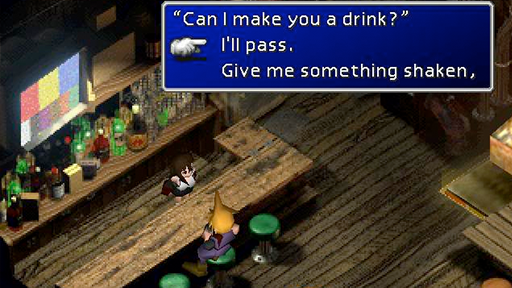
\includegraphics[width=\textwidth]{ch3_1_box.png}
    \caption{Final Fantasy VII (1997)}
    \centering
    \label{fig:ch3_1_box}
\end{figure}

\newpage

\subsection{Kołowy}

W ramach tego systemu mowa o klasycznym wyświetlaniu napisów wspomagających dialog (tzn. mowa o
transkrypcji kwestii wypowiadanych przez postacie, a dokładniej przez aktorów głosowych). Pojęcie
koła pojawia się w momencie podejmowania przez gracza decyzji gdzie opcje ułożone w ogólnym
rozumieniu w okręgu (Patrz rys. \ref{fig:ch3_1_wheel}). Może to być podejście głównie znane
z gier wspierających konsole, ze względu na analagowe gałki w~kontrolerach, za pomocą których
łatwo wybrać odpowiednią pozycję.

\begin{figure}[h]
    \centering
    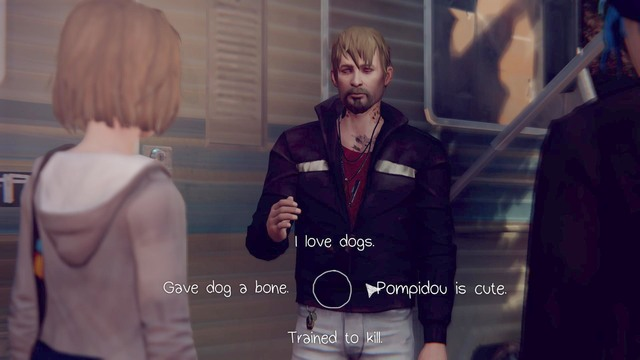
\includegraphics[width=0.9\textwidth]{ch3_1_lis.png}
    \caption{Life is Strange (2015)}
    \label{fig:ch3_1_wheel}
\end{figure}

\newpage

\subsection{Precyzjne / nieprecyzyjne}\label{subsubsection:ch3_1_precision}

Jak wspomniano na początku sekcji, precyzja określa pokrycie wyświetlanych opcji dialogowych z
faktycznymi kwestiami wypowiadanymi przez postać. Niektóre tytuły są krytykowane właśnie za
niezrozumiałe czy też nieintuicyjne wybory stawiane przed graczem. Przykładowo, w ramach gry
"Fallout 4" mamy do czynienia z bardzo krótkimi 1-3 słownymi komunikatami, które nie oddają
do końcu tonu i intencji wypowiedzi. Społeczność fanowska utworzyła nawet modyfikację do gry,
która zamienia kołowe i lakoniczne opcje na listę wyborów w formie zdań
(Patrz rys. \ref{fig:ch3_1_precision}).

\begin{figure}[h]
    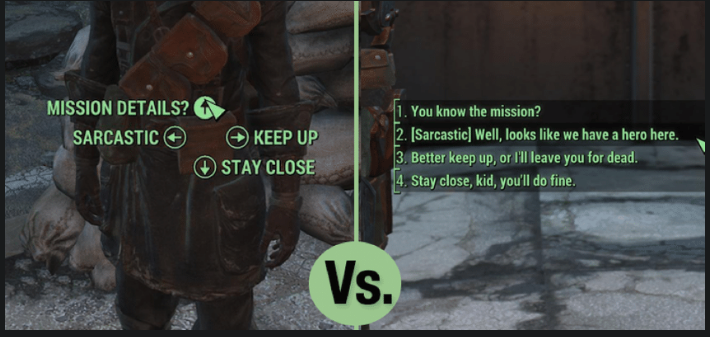
\includegraphics[width=\textwidth]{ch3_1_precision.png}
    \caption{Fallout 4 (2015) + wersja zmodowana\cite{spoken_conversational_ai}}
    \centering
    \label{fig:ch3_1_precision}
\end{figure}

\newpage

\subsection{Wykorzystujące emocje}

Systemy dialogowe mogą dodatkowo zawierać informacje o nacechowaniu emocjonalnym wypowiedzi.
W grze "Dragon Age: Inquisition" można zaobserwować odpowiednie ikony, informujące grającego o
tym w jaki sposób sterowana przez gracza postać wypowie daną kwestię. Wycinek ikon wraz z ich
opisami został przedstawiony na rysunku \ref{fig:ch3_1_emotions_list}.

\begin{figure}[h]
    \centering
    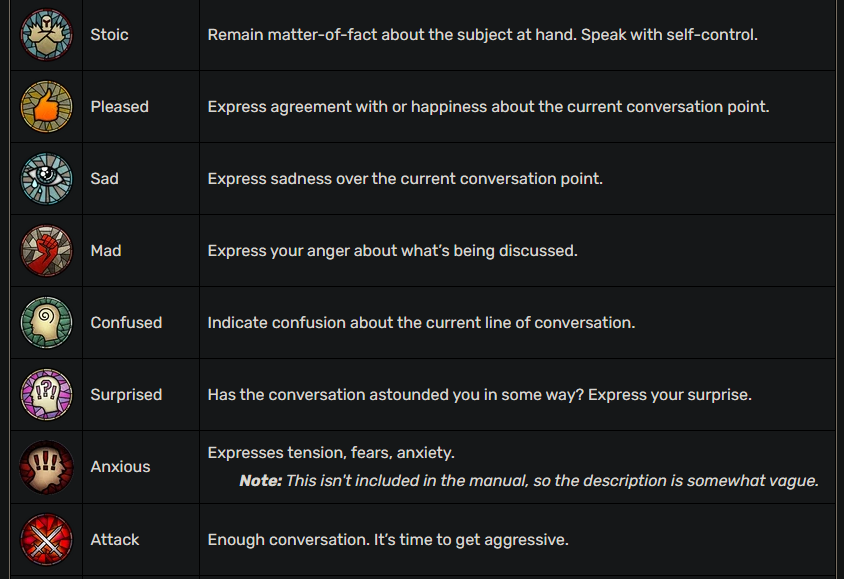
\includegraphics[width=0.8\textwidth]{ch3_1_emotions.png}
    \caption{Fragment spisu ikon dialogowych - "Dragon Age: Inquisition" (2014)\cite{dragon_age_fandom}}
    \label{fig:ch3_1_emotions_list}
\end{figure}

Ikony te są wyświetlane po najechaniu na odpowiednią opcję w momencie podejmowania decyzji
(Patrz rys. \ref{fig:ch3_1_emotions_example}).

\begin{figure}[h]
    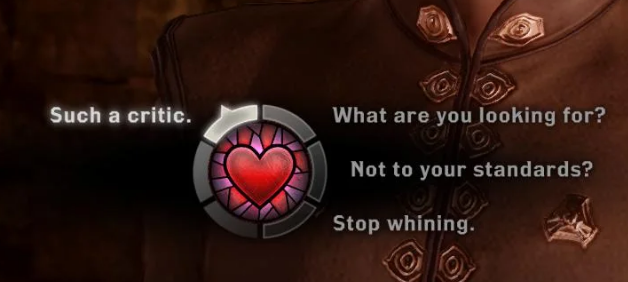
\includegraphics[width=\textwidth]{ch3_1_emotions2.png}
    \caption{Przykład dialogu z wykorzystaniem ikony emocji - "Dragon Age: Inquisition" (2014)}
    \centering
    \label{fig:ch3_1_emotions_example}
\end{figure}

\subsection{Wykorzystujące statystyki}

Niektóre tytuły, zwłaszcza te z gatunku \gls{rpg} (ang. \textit{role-playing game}) pozwalają rozwijać
statystyki czy też atrybuty postaci (np. siła, charyzma). W takich grach możemy napotkać się na
system dialogowy, w którym to pewne opcje są ograniczone czy też zablokowane ze względu na poziom
statystyk postaci sterowanej przez gracza. Przykładowo, w "Fallout: New Vegas" decyzje dialogowe
a co za tym idzie i fabularne, mogą ograniczać grającego do konkretnych rozwiązań
(Patrz rys. \ref{fig:ch3_1_stats}).

\begin{figure}[h]
    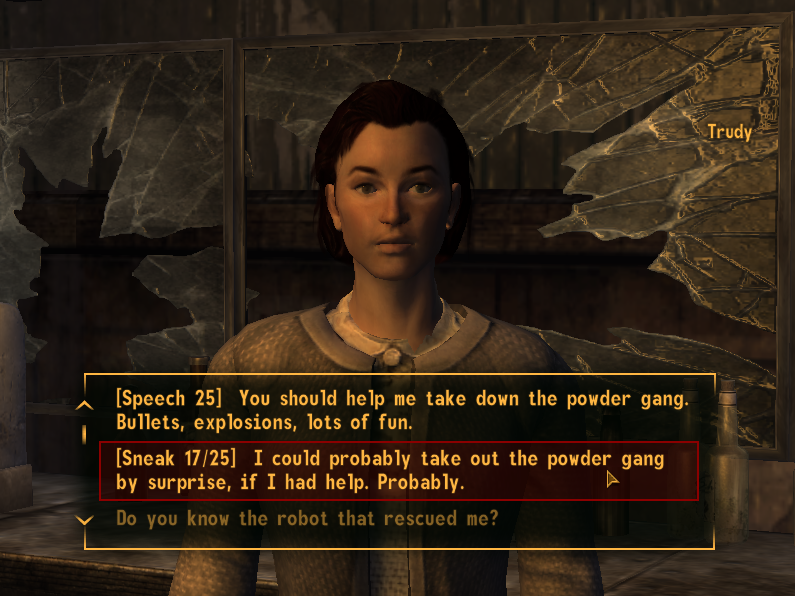
\includegraphics[width=\textwidth]{ch3_1_stats.png}
    \caption{Fallout: New Vegas (2010)}
    \centering
    \label{fig:ch3_1_stats}
\end{figure}

\newpage

\subsection{Wykorzystujące czas}

Spotykaną też czasami formą występującą w dialogach jest ograniczenie czasowe na podjęcie decyzji
narzucone na grającego przez grę. Jest to technika poniekąd inspirująca się metodą \gls{qte} znaną z
cut scenek (Patrz sekcja \ref{subsubsection:ch1_2_2_cutscene}). Rozwiązanie takie możemy znaleźć
w~grze "Wiedźmin 3" (Patrz rys. \ref{fig:ch3_1_time}). Jeśli gracz nie podejmie decyzji w
określonym czasie to albo kończy się to automatycznym wyborem jednej z dostępnych opcji albo
występuje de facto \textit{"trzecia opcja"}.

\begin{figure}[h]
    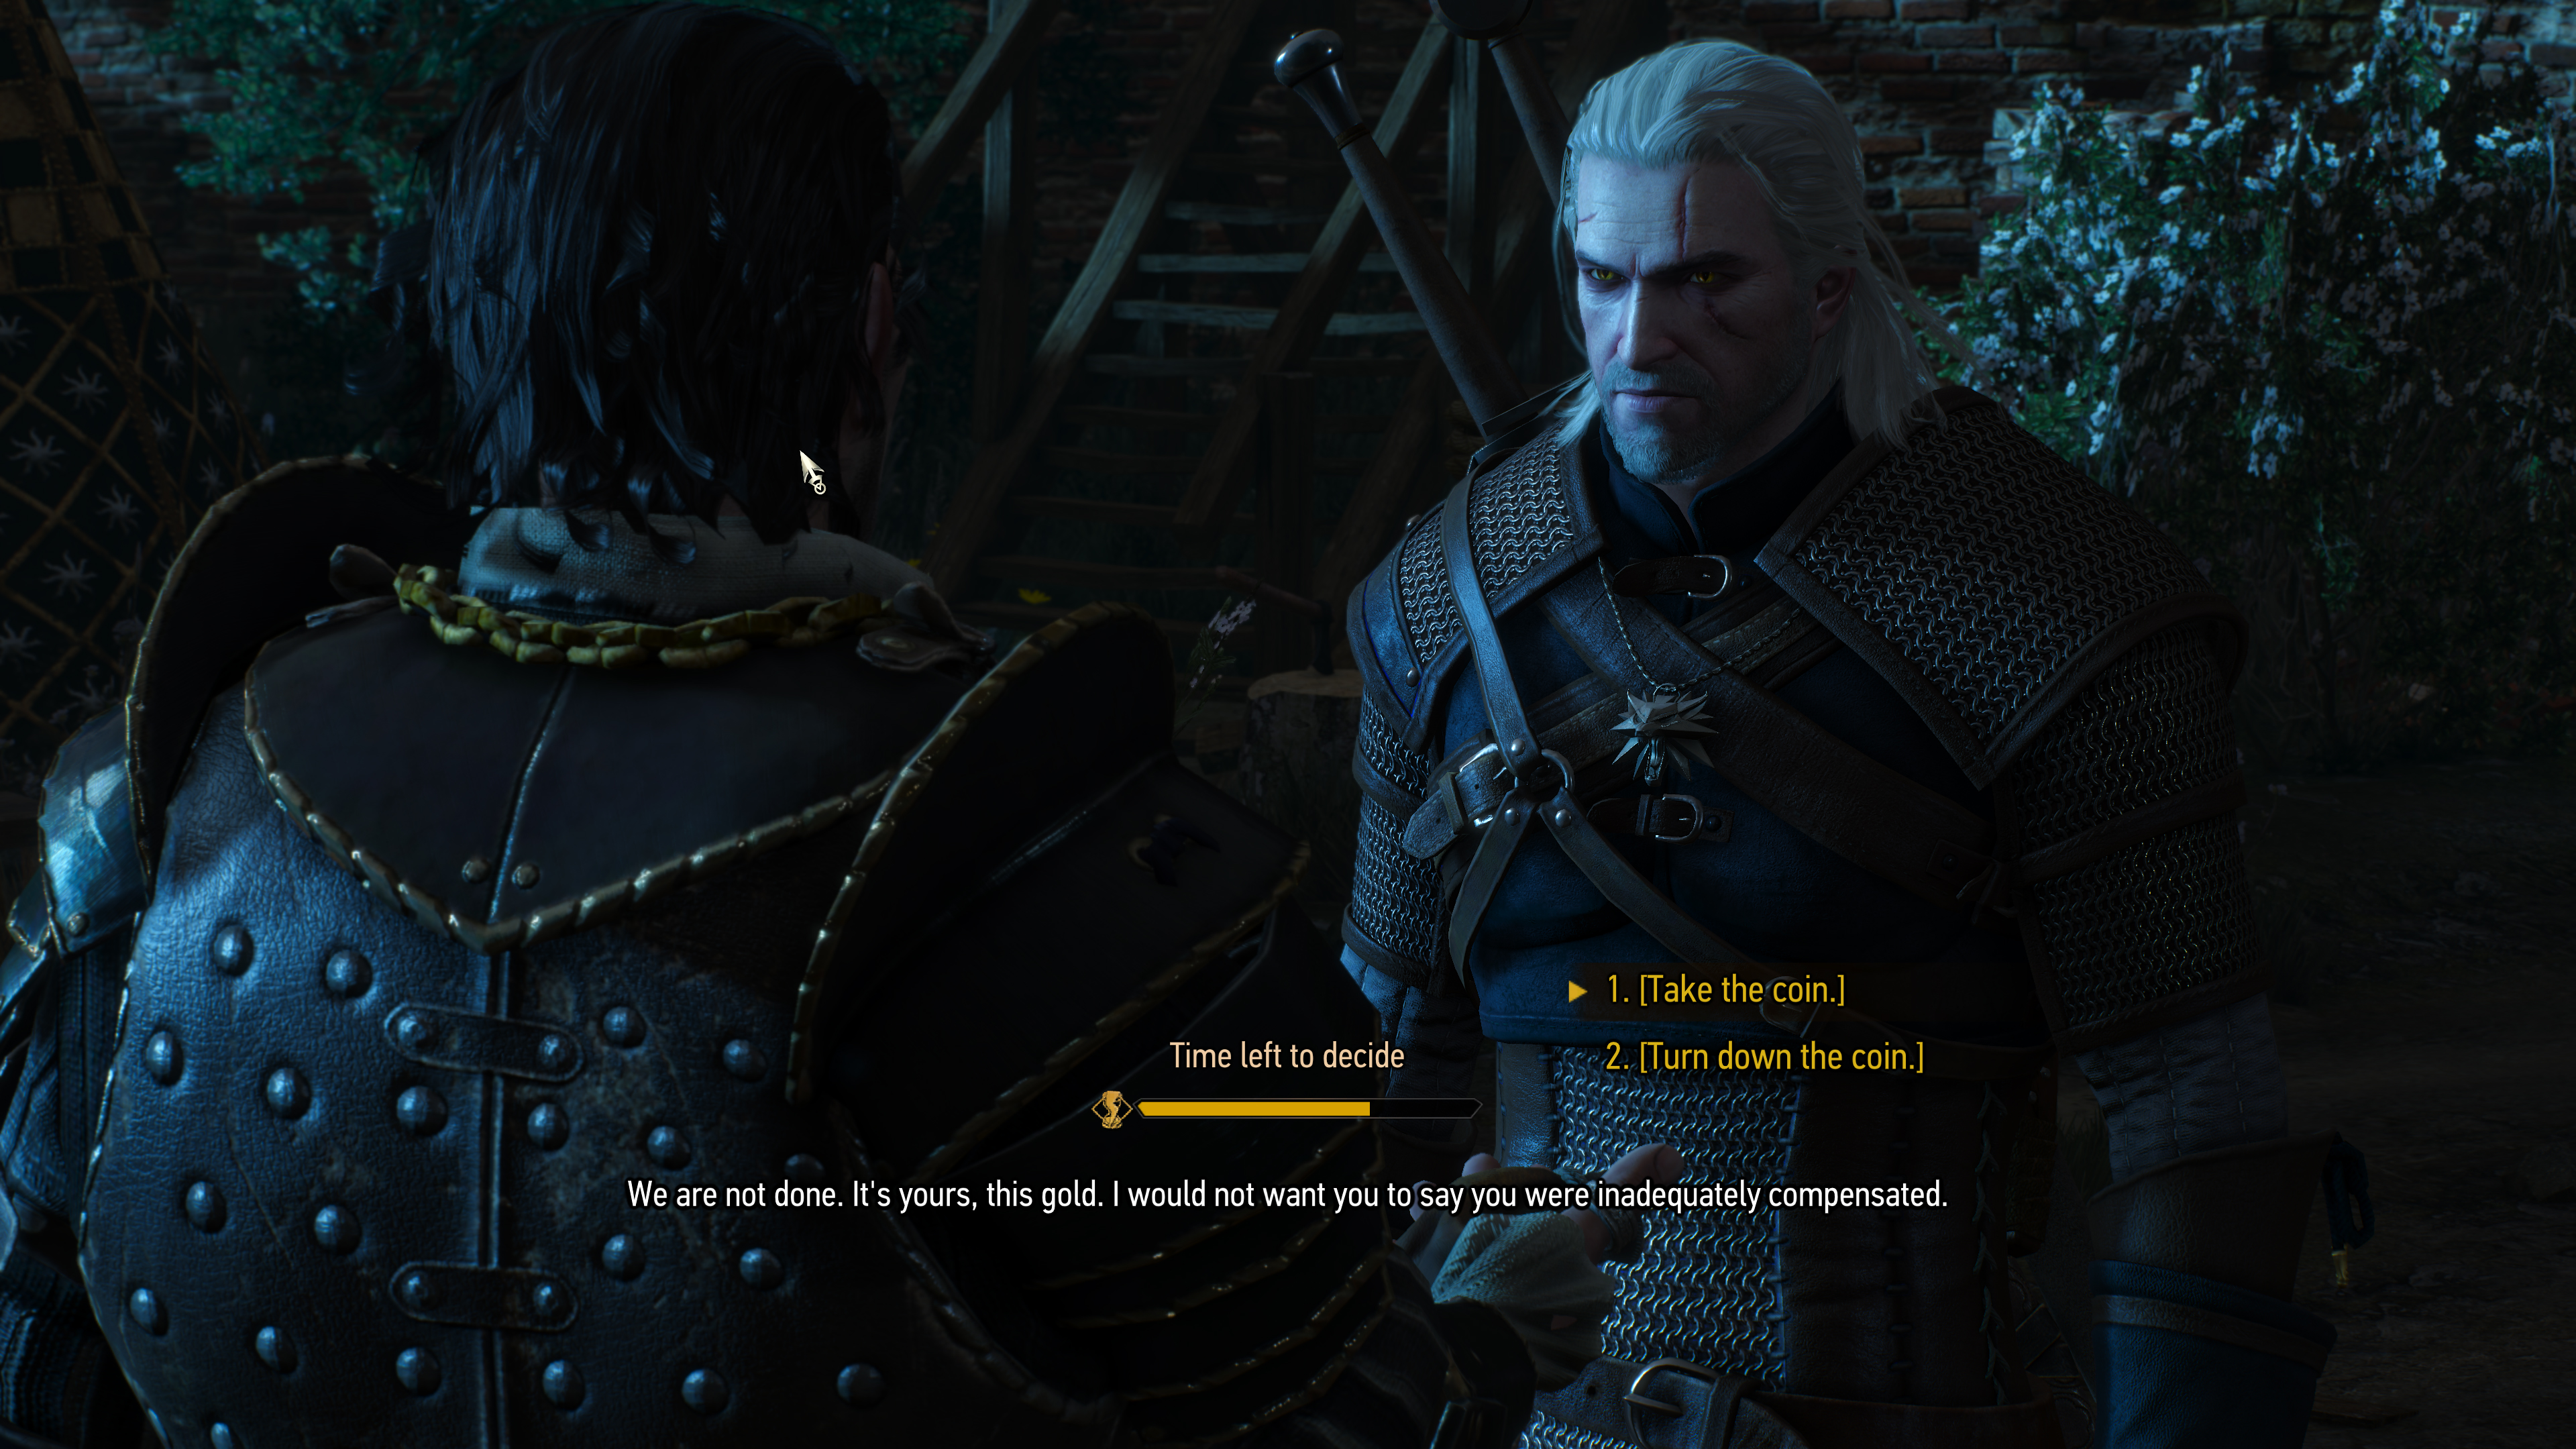
\includegraphics[width=\textwidth]{ch3_1witcher.png}
    \caption{Wiedźmin 3 (2015)}
    \centering
    \label{fig:ch3_1_time}
\end{figure}

\section{Interaktywna fikcja - system poleceń}\label{subsection:ch3_2}

Innego rodzaju systemem dialogowym --- a nawet i osobnym gatunkiem gier komputerowych --- jest
tak zwana \textit{interaktywna fikcja}. Jest ona pewnego rodzaju oprogramowaniem symulującym
środowisko, w którym to gracz używa wyłącznie komend tekstowych do poruszania się czy wpływania
na to środowisko\cite{if_wiki}. Według Nick'a Montfort'a pojęcie to może być utożsamione z
"przygodami tekstowymi" czy prościej "grami tekstowymi"\cite{IF_4th_era}. Z~perspektywy nauczania
maszynowego można uznać, że tego rodzaju gry zawierają w sobie elementy przetwarzania języka
naturalnego (z ang. \textit{\gls{nlp} - natural language processing}) jak i sekwencyjnego podejmowania
decyzji\cite{hausknecht2020interactive}. Przykład rozgrywki zostanie zaprezentowany w oparciu
o polski tytuł "Otchłań" (1999).

Po rozpoczęciu rozgrywki gracz znajduje się interaktywnym świecie gry, w którym różne kolory tekstu
mają specyficzne znaczenia, wskazujące na różne elementy rozgrywki. Błękitny tekst podobny do
\textbf{<21hp 104m 112mv 70exp>} oznacza status gracza, a sama gra oczekuje na polecenie.
Zielony tekst oznacza lokacje, w których znajduje się gracz, a różowy tekst wskazuje możliwe
wyjścia z danego miejsca. Krótkie opisy dają graczowi dodatkowe informacje o otoczeniu. Całość
tworzy spójną, interaktywną fabułę, w której gracz może podejmować decyzje i eksplorować świat gry.
Powyższe opisy są do zaobserwowania na rysunku \ref{fig:ch3_2_generic}.

\begin{figure}[h]
    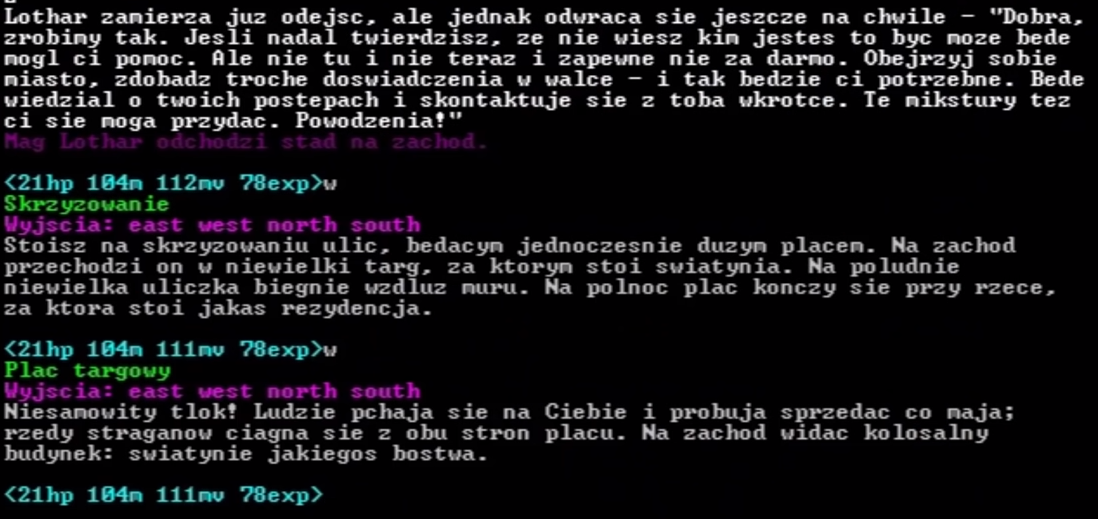
\includegraphics[width=\textwidth]{ch3_2_generic.png}
    \caption{Ogólny wygląd rozgrywki w "Otchłani"}
    \centering
    \label{fig:ch3_2_generic}
\end{figure}

Dialogi występujące w "Otchłani" z postaciami \gls{npc} prowadzone są w formie listy wybieralnych kwestii
z perfekcyjną precyzją (Patrz sekcja \ref{subsubsection:ch3_1_precision}), tzn. kwestia wypowiadana
jest w takiej formie, w jakiej występuja ona w menu. Sama konwersacja rozpoczynana jest oczywiście
za pomocą odpowiedniej komendy, a zakończona może być przez odpowiedni wybór użytkownika lub po
odpowiedzi od postaci \gls{npc} (co widać na rysunku \ref{fig:ch3_2_dialogue}).

\begin{figure}[h]
    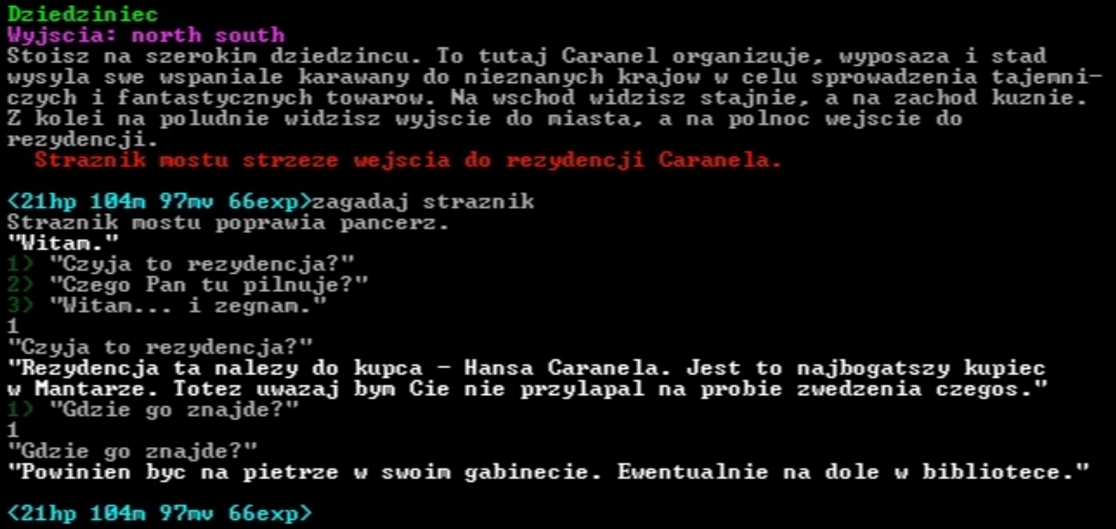
\includegraphics[width=\textwidth]{ch3_2_dialogue.png}
    \caption{Dialog w "Otchłani"}
    \centering
    \label{fig:ch3_2_dialogue}
\end{figure}

Gra oferuje pewnego rodzaju katalog dostępnych dla gracza poleceń, które pogrupowane są w
odpowiednie kategorie tematyczne. Aby uzyskać listę wystarczy wydać polecenie "pomoc". Mimo braku
szczegółowych opisów, komendy zostały zaprojektowane w formie dość intuicyjnych poleceń jako słowa
z języka polskiego. Pełna lista dostępnych komend jest widoczna na rysunku \ref{fig:ch3_2_commands}.

\begin{figure}[h]
    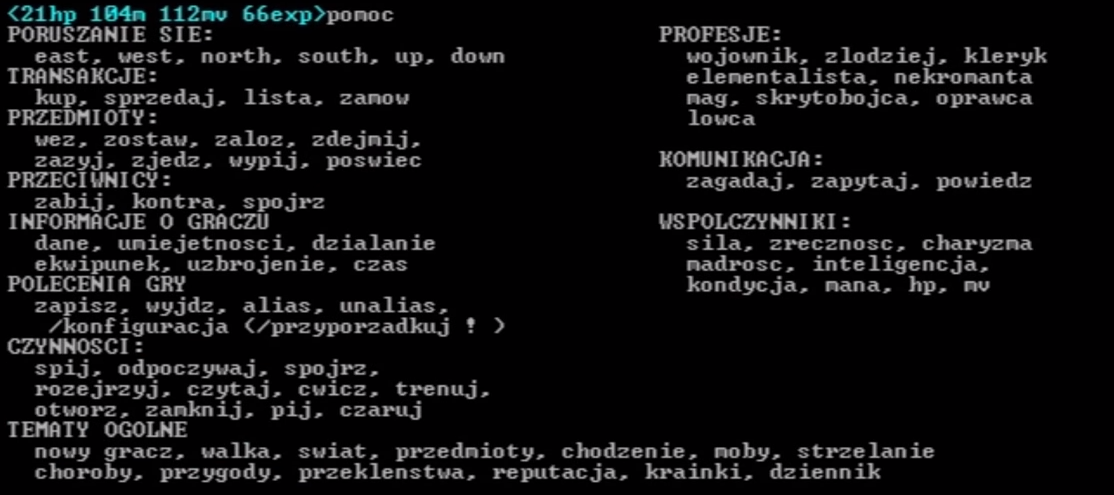
\includegraphics[width=\textwidth]{ch3_2_commands.png}
    \caption{Polecenia dostępne w "Otchłani"}
    \centering
    \label{fig:ch3_2_commands}
\end{figure}

W przypadku gdy grający ma problem ze zrozumieniem pewnych komend albo samego sposobu prowadzenia
rozgrywki to może sięgnąć po samouczek dostępny na oficjalnym forum "Otchłani". Na rysunku
\ref{fig:ch3_2_tutorial} zauważyć można szczegółowy opis komend związanych z kategorią
eksplorowania świata gry.

\begin{figure}[h]
    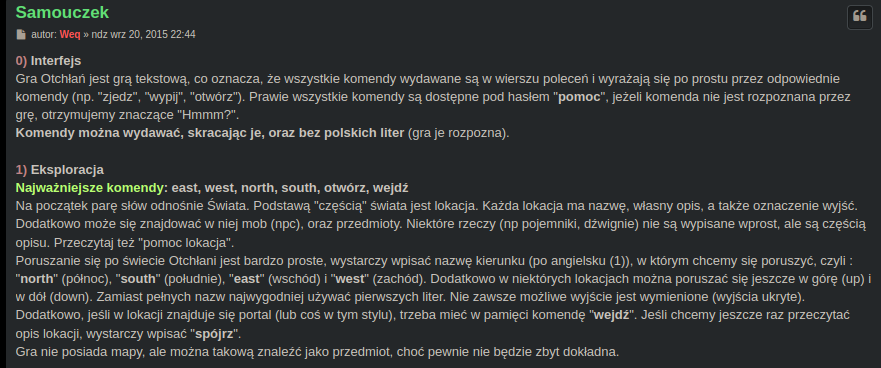
\includegraphics[width=\textwidth]{ch3_2_tutorial.png}
    \caption{Fragment samouczka "Otchłani"}
    \centering
    \label{fig:ch3_2_tutorial}
\end{figure}

W pracach nad "Otchłanią" zaangażowane były dwie osoby: Grzegorz 'Weq' Nowak oraz Krzysztof 'Hoborg'
Ciesielski. Zaczęli oni pracę nad grą w 1998 roku mając odpowiednio 16 i 14 lat\cite{otchlan_historia}.
Po kilku latach Krzysztof Ciesielski odszedł od projektu. Ostatecznie, Grzegorzowi Nowakowi udało się
po kilkunastu latach doprowadzić tytuł do wersji finalnej dostępnej za darmo na stronie
\href{https://www.otchlan.pl}{https://www.otchlan.pl}.